\documentclass[conference]{IEEEtran}
\IEEEoverridecommandlockouts
% The preceding line is only needed to identify funding in the first footnote. If that is unneeded, please comment it out.
\usepackage{cite}
\usepackage{amsmath,amssymb,amsfonts}
\usepackage{algorithmic}
\usepackage{graphicx}
\usepackage{textcomp}
\usepackage{xcolor}
\def\BibTeX{{\rm B\kern-.05em{\sc i\kern-.025em b}\kern-.08em
    T\kern-.1667em\lower.7ex\hbox{E}\kern-.125emX}}
\begin{document}

\title{Assumption of Bitcoin Regulation Using Extra Basic Data Structures \\
}

\author{\IEEEauthorblockN{1\textsuperscript{st} Liu Feng}
\IEEEauthorblockA{\textit{ECE Department} \\
\textit{Stevens Institute of Technology}\\
Hoboken, USA \\
fliu17@stevens.edu}
\and
\IEEEauthorblockN{1\textsuperscript{st} Wu Siyang}
\IEEEauthorblockA{\textit{ECE Department} \\
	\textit{Stevens Institute of Technology}\\
	Hoboken, USA \\
swu32@stevens.edu}
\and
\IEEEauthorblockN{1\textsuperscript{st} Xu Xiangyang}
\IEEEauthorblockA{\textit{ECE Department} \\
	\textit{Stevens Institute of Technology}\\
	Hoboken, USA \\
xxu46@stevens.edu}
}

\maketitle

\begin{abstract}
Bitcoin is a decentralized digital currency without any banks or administrators. Since Bitcoin can be sent from user to user with no intermediaries, we decide to conceive a manner for regulating it. After the study about Libra (a cryptocurrency which is similar with Bitcoin), we use some basic data structures (Hash Table and Array List) as the assistance and apply the SHA256 algorithm in our work. 
\end{abstract}

\begin{IEEEkeywords}
Bitcoin, regulating, Libra, data structures, SHA256
\end{IEEEkeywords}

\section{Introduction}
Bitcoin is a collection of concepts and technologies that form the basis of a digital money ecosystem.  Bitcoin is created through a process called "mining," which involves competing to find solutions to a mathematical problem while processing bitcoin transactions and it also has the protocol, which includes built-in algorithms that regulate the mining function across the network. Due to bitcoin’s diminishing rate of issuance, more and more company start to make their own cryptocurrency to take over Bitcoin’s status. [1]

Recently, there comes another virtual currency which is Libra, it is the project for which social media giant Facebook released the concept paper on 18 June 2019. To regulate Libra, Facebook lets Libra commit to open access to the blockchain, and open infrastructure, given that “open access ensures low barriers to entry and innovation and encourages healthy competition that benefits consumers.” [2]

In a degree, Bitcoin is similar with Libra. Even though the real incentive for Bitcoin was to avoid regulatory agencies, we still propose to use basic data structures and apply an algorithm to make it possible for regulation of Bitcoin.

\section{FUNCTION WITH DIAGRAMS}

\subsection{Create a Server by Using a ArrayList (Siyang Wu)}

Since the trade of Bitcoin needs no information of each user, it is very difficult for any institution to identify who made the deal. As far as we know, the blockchain of Bitcoin is consist of block nodes and the information inside each node is a string which containing cryptographic hash of the previous block, a timestamp, transaction data and a random number. And the Bitcoin user who can get the same result of the random number in the front block will get a reward and create a new block as the tail of the blockchain to record a current deal made by other Bitcoin users. However, this string is not enough for regulation and we need a server which can have a set of user’s information (Miner, Giver and Payee). By using this server, we can track and search any validated Bitcoin users to prevent those illegal transfers from the transaction platform of Bitcoin.

If we want to regulate the Bitcoin, we must force every Bitcoin user to offer some solid information such as real name, phone number and local address in their own account. Based on this idea, we can use an Array List as the core of the server to store each user’s account because the Array List has the high efficiency for searching every element inside itself. For example, if one of accounts of Bitcoin users is active, the server will match this account to every element of the Array List, if they match, this account can keep making the Bitcoin transfer or recording any Bitcoin deal made by others, if they can’t, the server will reject any requests from this account.

\begin{figure}[ht]
	\centering
	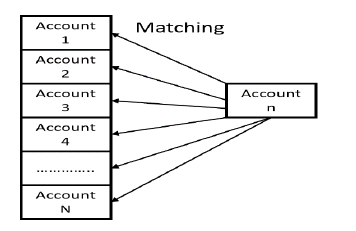
\includegraphics[scale=0.6]{fig1.png}
	\caption{Matcing in the Array List}
	\label{fig:label}
\end{figure}

\section{PSEUDO CODE}
\subsection{Server’s Part}
\begin{figure}[ht]	
	\centering
	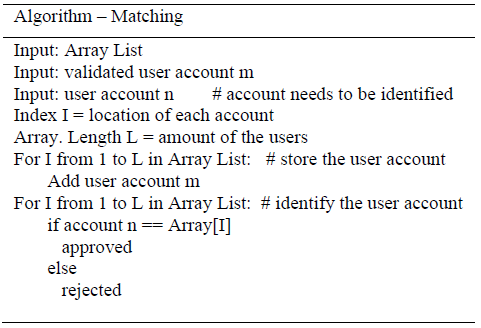
\includegraphics[scale=0.4]{ALG_M.png}
\end{figure}

\section{CONCLUSION}
Bitcoin is a decentralized cryptocurrency and has been criticized for its use in illegal transactions, its high electricity consumption, price volatility, and thefts from exchanges. Since the property of the blockchain of Bitcoin, it is very hard to modify any information of any transaction. However, if we use other extra basic data structures as a support to get an access to its blockchain just like what Facebook did to Libra, it will be regulated so how. In fact, it is impossible to fulfil the regulation of the Bitcoin and we hope our assumption can be applied to Bitcoin’s system one day.

\section{CONTRIBUTION}
In this work, Siyang Wu conceived the whole idea and composed the major part of this paper. Feng Liu has searched the algorithm for hash function and analyzed it. Xiangyang Xu has read the paper of the Libra and studied the property of the data structures we use.  

\begin{thebibliography}{00}
\bibitem{b1} Andreas Antonopolous (2014). Mastering bitcoin: Programming the Open Blockchain
\bibitem{b2} Zetzsche D.A, Buckley R.P, Arner D.W (2019). Regulating LIBRA: The Transformative Potential of Facebook’s Cryptocurrency and Possible Regulatory Responses
\bibitem{b3} Cormen, Thomas H.; Leiserson, Charles E.; Rivest, Ronald L.; Stein, Clifford (2009). Introduction to Algorithms (3rd ed.). Massachusetts Institute of Technology. pp. 253–280. ISBN 978-0-262-03384-8.
\end{thebibliography}
\end{document}


